%
% LaTeX report template 
%

% This is a comment: in LaTeX everything that in a line comes
% after a "%" symbol is treated as comment

\documentclass[11pt, a4paper]{article}
\usepackage{graphicx}
\usepackage{amsmath}
\usepackage{listings}


\title{EE2703 Endsemester Exam} % Title

\author{Prasanna Bartakke EE19B106} % Author name

\date{\today} % Date for the report
\begin{document}		
		
\maketitle % Insert the title, author and date
\section{Aim}
%Create new section;it is autonumbered
To find the variation of the magnetic field along the z-axis due to a circular loop of a wire with a given current centred at the origin.
\section{The Problem}
We have a loop of radius $a$, placed in $X-Y$ centred at the origin. The loop carries the current given below,
\begin{equation}\label{eq:1}
I = \frac{4\pi cos(\phi)exp(j\omega t)}{\mu_o}
\end{equation}
The following is the plot of the current.
\begin{figure}[!tbh]
   	\centering
   	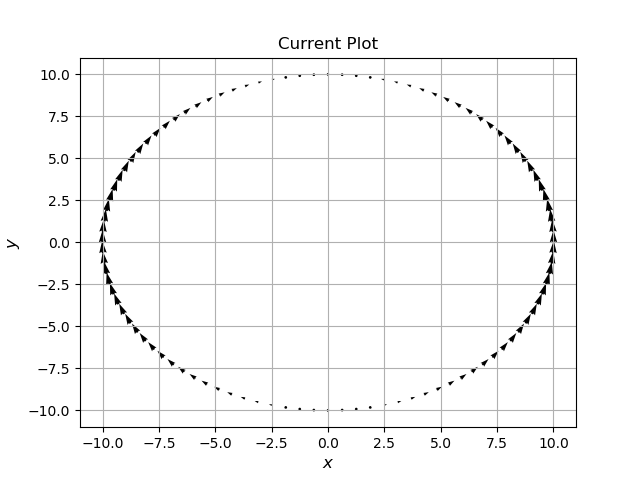
\includegraphics[scale=0.5]{fig1.png}  % Mention the image name within the curly braces. Image should be in the same folder as the tex file. 
   	\caption{Flow of current in the loop(case 1)}
   	\label{fig:sample}
   \end{figure} 
   
 As we can see the current is clockwise in one half and anticlockwise in other half of the loop. We can expect the magnetic field along the z axis, $B_z(0, 0, z)$ to be zero, as the magnetic field due to one half will get cancelled due to other half along z axis.
 
As we have to fit this curve to the given function, I have considered the case where current is anticlockwise in the entire loop. The equation for the current becomes,
\begin{equation}\label{eq:1}
I = \frac{4\pi |cos(\phi)| exp(j\omega t)}{\mu_o}
\end{equation}
The following is the plot of the current.
\begin{figure}[!tbh]
   	\centering
   	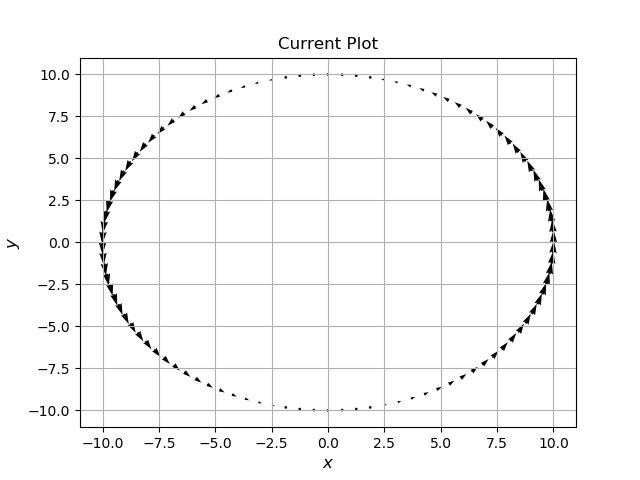
\includegraphics[scale=0.5]{fig4.png}  % Mention the image name within the curly braces. Image should be in the same folder as the tex file. 
   	\caption{Flow of current in the loop(case 2)}
   	\label{fig:sample}
   \end{figure}
For this configuration we can expect the magnetic field to be non zero along the z axis.
\newpage
\section{Logic}
Following is the graph of co-ordinate system.
\begin{figure}[!tbh]
   	\centering
   	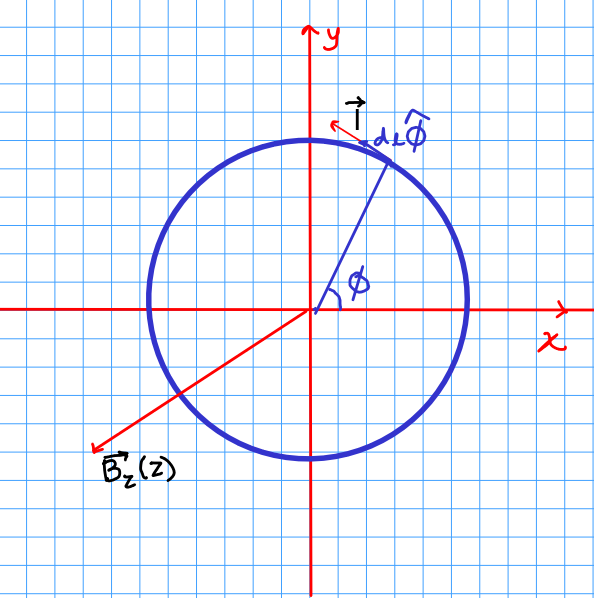
\includegraphics[scale=0.5]{figure.png}  % Mention the image name within the curly braces. Image should be in the same folder as the tex file. 
   	\caption{Relevant vectors}
   	\label{fig:sample}
   \end{figure}
 We can compute $\vec{A}$ using the formula,
 \begin{equation}\label{eq:1}
\vec{A}(r, \phi, z) = \frac{\mu_o}{4\pi}\int\frac{I(\phi)\hat{\phi}e^{-jkR}ad\phi}{R}
\end{equation}
where $\vec{R} = \vec{r} - \vec{r}^{'}$. $\vec{r}^{'}$ is the point on the loop.\\
We can simplify this to get the following result,
\begin{equation}\label{eq:1}
A_{ijkl}= \sum_{l=0}^{N-1}\frac{cos(\acute{\phi_{l}}) e^{-jkR_{ijkl}}\vec{d\acute{l}}}{R_{ijkl}}
\end{equation}\\

From $\vec{A}$ we can obtain $\vec{B}$ as follows,
\begin{equation}
\vec{B} = \nabla \times \vec{A}  
\end{equation}
\begin{equation}
Bz(z) = \frac{A_y(\Delta x,0,z) - A_x(0,\Delta y,z) - A_y(-\Delta x,0,z) + A_x(0,-\Delta y,z)}{4 \Delta x \Delta y}
\end{equation}
\newpage
\section{Pseudo Code}
\begin{description}
\item[$\bullet$]Divide the space into $3 \times 3 \times 1000$ grid with points separated by 1 cm. \\
\item[$\bullet$]Break the loop into 100 parts. $\phi$ : 100 divisions from 0 to $2\pi$.\\
\item[$\bullet$]$r_{ijk}$ contains the vector positions for which we want to compute $\vec{A}, \vec{B}$.\\
\item[$\bullet$]$r\textunderscore$ corresponds to the points $(a\cos(\phi), a\sin(\phi), 0)$ on the loop.\\
\item[$\bullet$]Calculate $R_{ijkl} = |r_{ijkl} - r\__{l}|$\\
\item[$\bullet$]Calculate $\vec{A}$ according to equation 4.\\
\item[$\bullet$]Calculate $\vec{B}$ according to equation 5.\\
\item[$\bullet$]Plot $\vec{B}$ vs $z$.
\item[$\bullet$]Fit B to the curve $cz^b$.
\end{description}

\section{Break the volume}
We need to break the volume into a 3 by 3 by 1000 points mesh, with mesh points separated by 1 cm.
This is done by the code below:
\begin{lstlisting}	
def create_points():
	#generate x, y, z coordinates of all the required points
	x = arange(-1, 2, 1)
	y = arange(-1, 2, 1)
	z = arange(1,1001,1)

	X, Y, Z = meshgrid(x,y,z)
	r = zeros((3,3,1000,3))
	r[:,:,:,0] = X
	r[:,:,:,1] = Y
	r[:,:,:,2] = Z
	return x, y, z, r
\end{lstlisting}

\section{Break the loop}
We need to break the loop into 100 sections. It is done by the code given below.
\begin{lstlisting}
def create_loop_locations():
	#r_ contains coordinates of the sections of the loop 
	rx = expand_dims(a * cos(phi), axis = -1)
	ry = expand_dims(a * sin(phi), axis = -1)
	rz = expand_dims(zeros(N), axis = -1)
	r_ = hstack((rx, ry, rz))
	return r_
\end{lstlisting}


Following figure represents the  locations of these 100 sections on the loop.
\begin{figure}[!tbh]
   	\centering
   	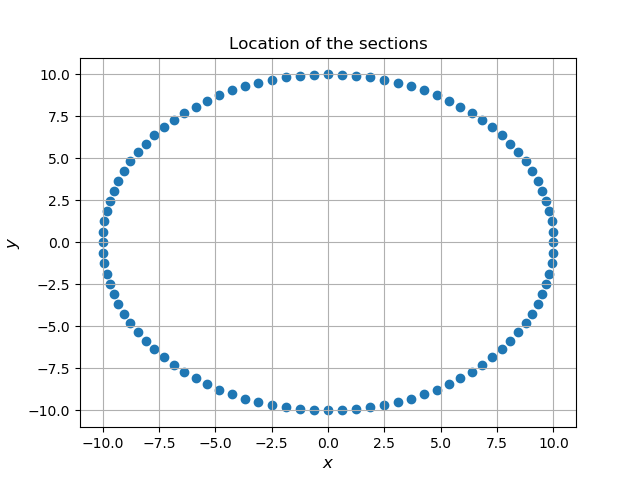
\includegraphics[scale=0.5]{fig0.png}  % Mention the image name within the curly braces. Image should be in the same folder as the tex file. 
   	\caption{Relevant vectors}
   	\label{fig:sample}
   \end{figure}


\section{Obtain $\vec{dl}^{'}$}
Following code is used to get $\vec{dl}^{'}$ = $dl \hat{\phi}$.
\begin{lstlisting}
def create_dl_bar():
	dl=2*np.pi*10/N*vstack((-sin(phi), cos(phi))) 
	dl = dl.T
	return dl
\end{lstlisting}

\section{Calculate R}
Following function calc() is used to calculate $\vec{R}_{ijkl} = |\vec{r}_{ijk} - \vec{r}^{'}_{l}|$
\begin{lstlisting}
def calc(l):
	return norm(r - r_[l], axis=-1)
\end{lstlisting}

\section{Calculate $\vec{A}, \vec{B}$}
Till now all the steps were same for both the cases. To calculate $\vec{A}, \vec{B}$ we need to do appropriate changes in both cases.
\subsection{Case 1 : Current given in equation 1}
\subsubsection{$\vec{A}$}
The following code is used to calculate $\vec{A}$.\\
\begin{lstlisting}
def calc_extended(l):
	R=norm(tile(r, 100).reshape(3, 3, 1000, 100, 3)-r_, axis=-1)   
	ai = sum(cos(phi) * exp(-1j * R/10) * dl[:,l] / R, axis = -1)
	return ai

def calculate_A():
	A = zeros((3,3,1000,2), dtype=complex) 
	for l in range(2):
		A[:,:,:, l] = calc_extended(l)
	return A

\end{lstlisting}
\subsubsection{$\vec{B}$}
Using this $\vec{A}$, we calculate  $\vec{B}$ using the following code.
\begin{lstlisting}
Bz = (A[1, 2, :, 1] - A[2, 1, :, 0] - A[1, 0, :, 1] + A[0, 1, :, 0]) / 4
\end{lstlisting}

\subsubsection{Plot Bz vs z}
\begin{figure}[!tbh]
   	\centering
   	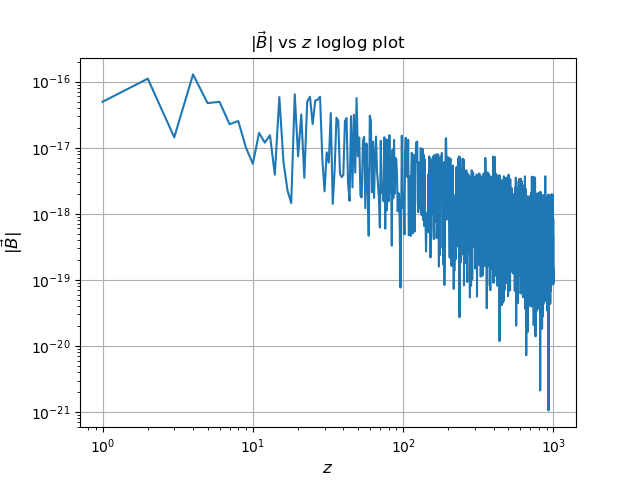
\includegraphics[scale=0.5]{fig2.png}  % Mention the image name within the curly braces. Image should be in the same folder as the tex file. 
   	\caption{Plot of Bz vs z.}
   	\label{fig:sample}
   \end{figure}
As expected we get $\vec{B}$ equal to zero throughout the z axis. The extremely small values of $\vec{B}$ are due the limited precision.

\newpage
\subsection{Case 2 : Current given in equation 2}
\subsubsection{$\vec{A}$}
The following code is used to calculate $\vec{A}$.\\
\begin{lstlisting}
def calc_extended1(l):
	R=norm(tile(r, 100).reshape(3, 3, 1000, 100, 3)-r_, axis=-1)   
	ai = sum(abs(cos(phi))*exp(-1j*R/10)*dl[:,l]/R, axis = -1)
	return ai

def calculate_A1():
	A = zeros((3,3,1000,2), dtype=complex)
	for l in range(2):
		A[:,:,:, l] = calc_extended1(l)
	return A

\end{lstlisting}
\subsubsection{$\vec{B}$}
Using this $\vec{A}$, we calculate $\vec{B}$ using the following code.
\begin{lstlisting}
Bz = (A[1, 2, :, 1] - A[2, 1, :, 0] - A[1, 0, :, 1] + A[0, 1, :, 0]) / 4
\end{lstlisting}

\subsubsection{Plot Bz vs z}
\begin{figure}[!tbh]
   	\centering
   	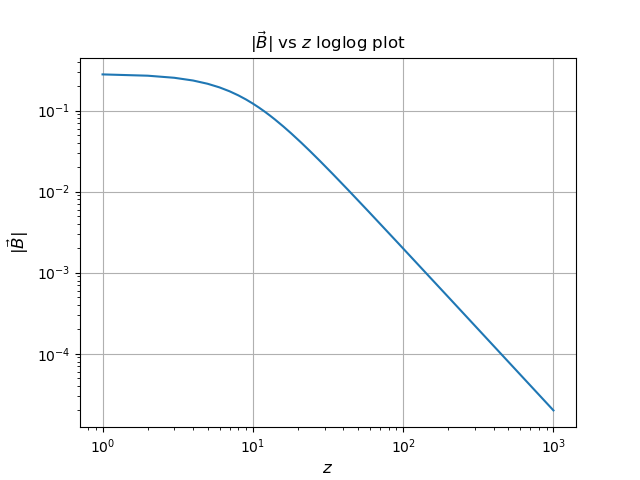
\includegraphics[scale=0.5]{fig5.png}  % Mention the image name within the curly braces. Image should be in the same folder as the tex file. 
   	\caption{Plot of Bz vs z.}
   	\label{fig:sample}
   \end{figure}
We get the following plot of $\vec{B}$ which is as expected.

\subsubsection{Approximating the magnetic field}
The function used to approximate the magnetic field $B_z(z)$ is $f(z) = cz^b$. We have to find the values of the parameters b, c.
\\We solve this problem by the least squares method. We can take log on both sides and attempt to fit the function as follows:
\begin{equation}
log(B_z(z)) = log(f(z)) = b * log(z) + log(c)
\end{equation}
This becomes a linear fit problem now. We can use the numpy.linalg.lstsq module to solve this problem.
Following is the code:
\begin{lstlisting}
def fit(Bz):
	a = hstack([ones(len(Bz[k : ]))[:,np.newaxis],
	log(z[k : ])[:,np.newaxis]])
	log_c, b = lstsq(a, log(abs(Bz[k : ])), rcond = None)[0]
	c = exp(log_c)
	return c, b
\end{lstlisting}
We try to fit the function for values of z after the theshold k.
I have used k = 50 for approximating the coefficients. The approximate graph obtained is given below.\\

\begin{figure}[!tbh]
   	\centering
   	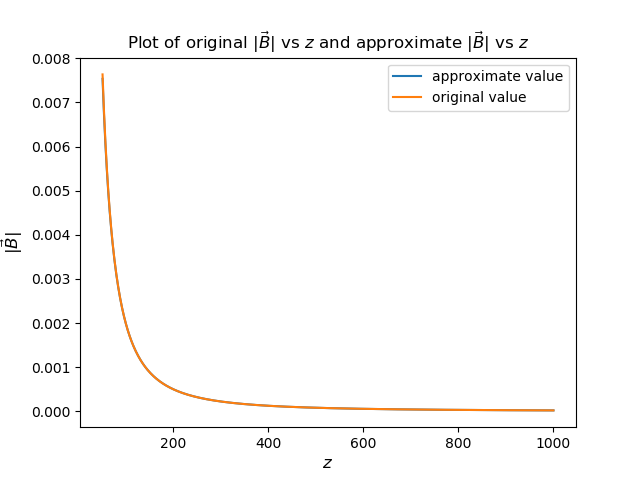
\includegraphics[scale=0.5]{fig6.png}  % Mention the image name within the curly braces. Image should be in the same folder as the tex file. 
   	\caption{Approximate graph along with original graph}
   	\label{fig:sample}
   \end{figure}
   As we can see, the approximate graph is almost equal to the original graph for all values of z. We note that b is -2. Thus we can see that the magnetic field falls proportional to inverse sqaure of z.
\newpage
\section{Comparing results with the static case}
Using Biot-Savart's law, the magnetic field along z axis is given as follows:
\begin{equation}
B_z(z) = \frac{2a^2}{(z^2 + a^2)^{3/2}}
\end{equation}
Thus we can see that $B_z(z)$ varies as $z^{-3}$. This difference arises due to the exponential term in the current $exp(-jwt)$.


\section{Conclusion}
In this assignment we studied the vector potential $\vec{A}$ and magnetic field $\vec{B}$ due to a current carrying loop.\\
We attempted to fit the function $cz^b$ to the obtained magnetic field.\\
We observed that $B_z$ varies as $z^{-2}$ for the given current, whereas in the statics case the vield varies as  $z^{-3}$. 
\end{document}


 